\documentclass[conference]{IEEEtran}
\usepackage{cite}
\usepackage{amsmath,amssymb,amsfonts}
\usepackage{algorithmic}
\usepackage{graphicx}
\usepackage{siunitx}
\usepackage{textcomp}
\usepackage{xcolor}
\usepackage{multirow}
\usepackage{url}
\usepackage{listings}
\usepackage{epstopdf}
\usepackage{subcaption}
\usepackage[inkscapeformat=png]{svg}
\usepackage[font=small,labelfont=bf]{caption}

\epstopdfDeclareGraphicsRule{.gif}{png}{.png}{convert gif:#1 png:\OutputFile}
\AppendGraphicsExtensions{.gif}

\begin{document}

\title{Using Generative Neural Networks to generate artist-inspired artwork}

\author{
    \IEEEauthorblockN{Mihai Bojescu}
    \IEEEauthorblockA{
        \textit{Master in Artificial Intelligence and optimisation}\\
        \textit{Faculty of Computer Science}\\
        \textit{University ``Alexandru Ioan Cuza'' of Iași}\\
        Iași, Romania \\
        bojescu.mihai@gmail.com
    }
    \and
    \IEEEauthorblockN{Radu Șolcă}
    \IEEEauthorblockA{
        \textit{Master in Artificial Intelligence and optimisation}\\
        \textit{Faculty of Computer Science}\\
        \textit{University ``Alexandru Ioan Cuza'' of Iași}\\
        Iași, Romania \\
        radu.ssolca@gmail.com
    }
}
\maketitle

\begin{abstract}
    This document contains a study on how Generative Neural Networks could be applied in order to transform noise into artwork
    inspired by renoun artists. The architecture of the Network consists of a Convolutional Neural Network for the discriminator
    and a U-Net Convolutional Neural Network for the genetrator. The data on which the network is trained is a dataset with
    faimous paintings by Jean Monnet.   
\end{abstract}

\begin{IEEEkeywords}
    Generative Neural Networks, GANs, Convolutional Neural Networks, U-Nets.
\end{IEEEkeywords}

\section{Introduction}
    In this document, we will study how GANs could be used to generate pieces of art in the Jean Monnet style. GANs have shown
remarkable success in generating realistic images by using random noise as input, and we aim to use them as an application
for producing fine art.

    Monnet's paintings are characterised by their vibrant colors and expressive brushwork, and we will try to replicate this
signature in the pictures that the GAN produces, effectively creating a 'digital Monnet'. The model will play by rotation
the role of an art critic and an artist in order to improve itself until - as an art critic - it cannot distinguish between
real, pre-existing art and newly created art.

\section{Data processing}
    In our project, we have used only a resize transformation, which resizes the images from 256x256 to 32x32.

\section{GANs}
    Generative Adversarial Networks, a type of Neural Network that was originally built in 2014 by Ian Goodfellow and his
colleagues in June 2014 \cite{b1} is a type of machine learning system that involves two neural networks competing against
each other. The competition can be seen a game where two teams have to play a zero-sum game: one team's win is the other
team's loss. The system is part of the unsupervised learning category, but can also be used for semi-supervised learning,
fully-supervised learning and for reinforcement learning. The alforementioned system can be used for a vast set of use-cases,
ranging from image generation - the classical use-case - to music generation.

    GANs are known to produce high-quality results with good performance, but suffer of low diversity.

\begin{figure}[!h]
    \centering
    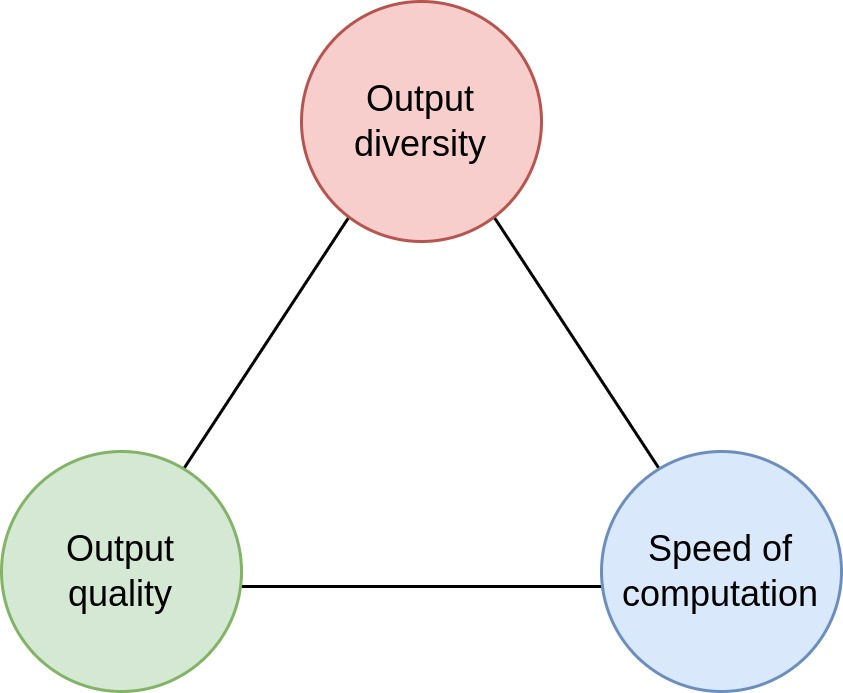
\includegraphics[scale=0.25]{images/generator problem.jpg}
    \caption{Data generation problem} \label{Data generation problem}
\end{figure}

    In our paper, we present a classical use-case for GANs: image generation. As seed, we will be using random noise from
the uniform distribution and we will use the seed to generate art in the Monet style.

\subsection{Discriminator}
    For a discriminator, we will use a classical cone-shaped convolutional neural network that receives an image with 3 channels
and in turn creates, 64, 128, 256, 512 feature maps, which are later flattened to a 1-dimensional array. The network makes use
of a Leaky Rectified Linear Unit activation function for the feature maps building, and a Sigmoid activation function at its
output.

    The trainer of the discriminator uses - for each time it is used - a batch of real images and a batch of fake ones, which are used
to ``teach'' the model how to classify images: fake ones are considered negative, while real ones as positive. For training we use
the Wasserstein distance - also named Earth Mover's distance - to compute the loss of the discriminator \cite{b2}:

\begin{multline}
    loss_{D} = - \frac{\sum_{i=0}^{n} discriminator\_output_{real\_image}^i}{n} \\
               + \frac{\sum_{i=0}^{n} discriminator\_output_{fake\_image}^i}{n} \\
               + gradient\_loss(fake\_image, real\_image)
\end{multline}

    Where $gradient\_loss$ is a function that computes, given a real and a fake image, a penalty that encourages the gradients
of the critic to have norm 1 almost everywhere. This is used in order to enforce the Lipschitz continuity constraint, which
in turn should improve the results.

\subsection{Generator}
    The generator of the GAN is comprised of a classical U-Net architectured CNN. U-Nets are well known for producing pictures
with the same shape as the input, which in our case proved beneficial, as we could provide noise for each pixel of the image,
noise. After training, the generator \textit{should} output realistic-looking Monet-inspired pictures.

    For its architecture, we used multiple layers of convolutional and max-pooling layers that downscale the image and extract features,
data which is later used to upscale the image back using multiple transposed convolutional and classical convolutional layers.
For the activation function we also use the Leaky Rectified Linear Unit function.

    The trainer performs the following steps for the generator:
\begin{enumerate}
    \item Using a given noise tensor, run the generator
    \item Using the output of the generator, run the discriminator
    \item Use the inverted results of the discriminator to update the loss of the generator
\end{enumerate}

\begin{multline}
    loss_{G} = - \frac{\sum_{i=0}^{n} discriminator\_output_{fake\_image}^i}{n}
\end{multline}

\section{Shortfalls}
    GANs are well-known for being unstable in training, and are also well-known for suffering of the mode collapse problem -
learning so well the training data of the discriminator, that it becomes a generator that outputs only the training data. In
our case, the diversite issue was mitigated by using the gradient penalty function. The model proved to be highly unstable,
most often outputting noise.

\section{Results}
    In general, most of the results could not be distinguished from the random noise used to generate the generator's outputs
(\ref{noisy sample}, \ref{noisy sample 2}). The red in the discriminator output means that the discriminator classified the
output of the generator as a fake image. There were results where some shapes could be distinguished, but they were not close
to the original paintings (\ref{sample with shape}, \ref{sample with shape 2}).

    We trained our model on an Intel Core i7 1260p processor, a NVIDIA RTX 3070Ti laptop GPU and a NVIDIA T4 GPU in the cloud.
We collected the following metrics from our training runs:

\begin{table}[!h]
    \centering
    \begin{tabular}{|c|c|}
        \hline
        Processor & Mean timing per iteration \\
        \hline
        Intel i7 1260p & 12s \\
        NVIDIA RTX 3070Ti & 1.3s \\
        NVIDIA T4 & 1.83s \\
        \hline
    \end{tabular}
    \caption{Performance metrics} \label{performance metrics}
\end{table}

\section{Conclusions}
    In literrature, GANs can be used to generate art from random noise. In our project we aimed to replicate these results,
but at best we could generate only shaped artifacts. The model would need further debugging and fine-tuning before it can
generate meaningful data.

\begin{thebibliography}{00}
    \bibitem{b1} I. J. Goodfellow, J. Pouget-Abadie, M. Mirza, B. Xu, D. Warde-Farley, S. Ozair, A. Courville, Y. Bengie
    (2014). ``Generative Adversarial Nets''. Département d'informatique et de recherche opérationnelle Université de Montréal
    Montréal, QC H3C 3J7. arXiv: 1406.2661v1
    \bibitem{b2} M. Arjovsky, S. Chintala, L. Bottou (2017). ``Wasserstein GAN''. Courant Institute of Mathematical Sciences.
    arXiv: 1701.07875v3
\end{thebibliography}

\begin{figure}[!h]
    \centering
    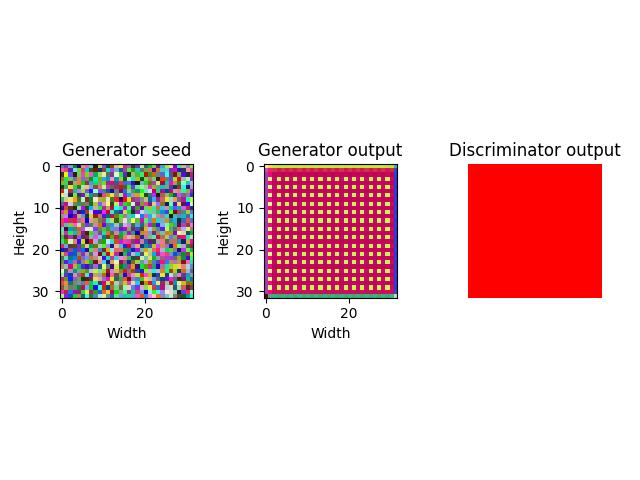
\includegraphics[scale=0.20]{images/noisy sample.jpg}
    \caption{Noisy sample} \label{noisy sample}
    \centering
    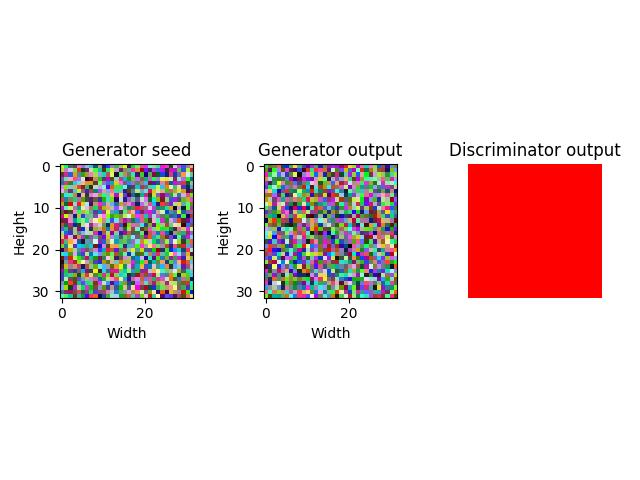
\includegraphics[scale=0.20]{images/noisy sample 2.jpg}
    \caption{Noisy sample 2} \label{noisy sample 2}
\end{figure}

\begin{figure}[!h]
    \centering
    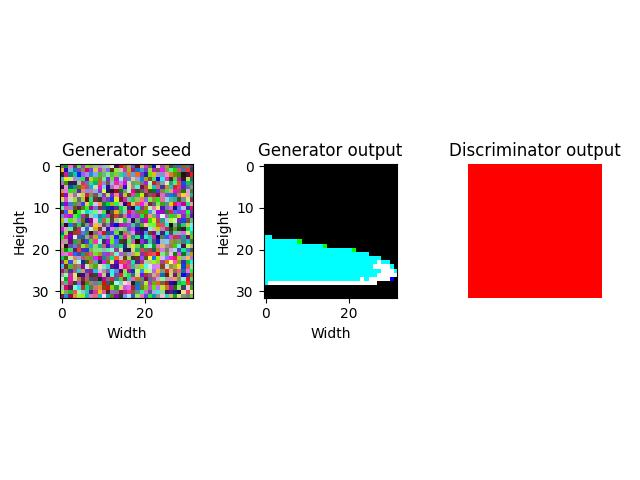
\includegraphics[scale=0.15]{images/sample with shape.jpg}
    \caption{Sample with shape} \label{sample with shape}
    \centering
    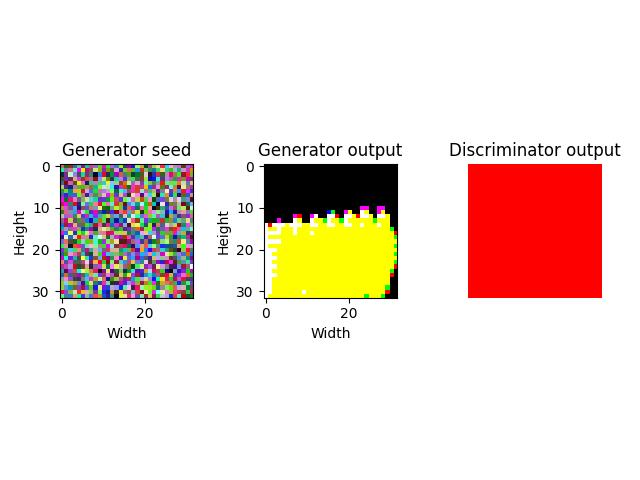
\includegraphics[scale=0.15]{images/sample with shape 2.jpg}
    \caption{Sample with shape 2} \label{sample with shape 2}
\end{figure}

\end{document}
